% Figure 1: System Architecture Diagram
% This figure shows the layered architecture of AetherLog 2.0

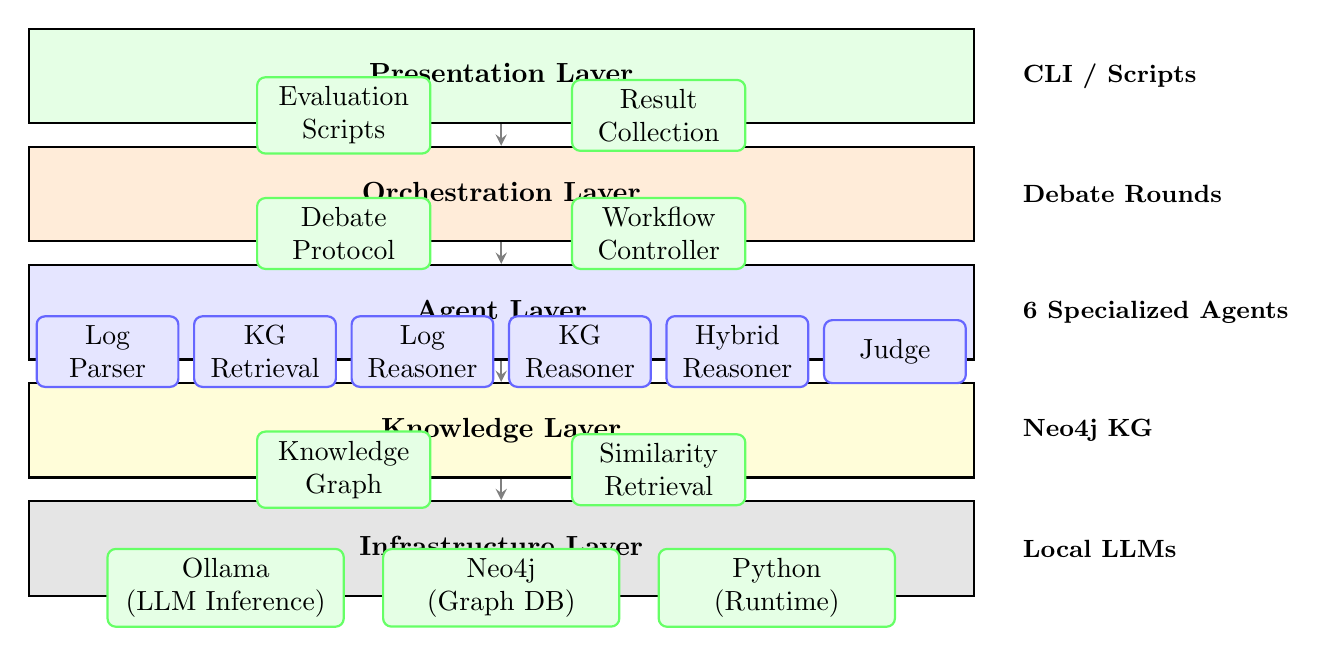
\begin{tikzpicture}[
    node distance=0.8cm,
    layer/.style={rectangle, draw=black, thick, minimum width=12cm, minimum height=1.2cm, align=center},
    agent/.style={rectangle, draw=blue!60, fill=blue!10, thick, minimum width=2.5cm, minimum height=0.8cm, align=center, rounded corners=3pt},
    component/.style={rectangle, draw=green!60, fill=green!10, thick, minimum width=2.2cm, minimum height=0.7cm, align=center, rounded corners=3pt},
    arrow/.style={->, thick, >=stealth},
    label/.style={font=\small\bfseries}
]

% Layers (bottom to top)
\node[layer, fill=gray!20] (infra) at (0,0) {\textbf{Infrastructure Layer}};
\node[layer, fill=yellow!15] (knowledge) at (0,1.5) {\textbf{Knowledge Layer}};
\node[layer, fill=blue!10] (agent) at (0,3) {\textbf{Agent Layer}};
\node[layer, fill=orange!15] (orch) at (0,4.5) {\textbf{Orchestration Layer}};
\node[layer, fill=green!10] (pres) at (0,6) {\textbf{Presentation Layer}};

% Infrastructure components
\node[component, minimum width=3cm] (ollama) at (-3.5,-0.5) {Ollama\\(LLM Inference)};
\node[component, minimum width=3cm] (neo4j) at (0,-0.5) {Neo4j\\(Graph DB)};
\node[component, minimum width=3cm] (python) at (3.5,-0.5) {Python\\(Runtime)};

% Knowledge layer components
\node[component] (kg) at (-2,1) {Knowledge\\Graph};
\node[component] (retrieval) at (2,1) {Similarity\\Retrieval};

% Agent layer - 6 agents
\node[agent, minimum width=1.8cm] (parser) at (-5,2.5) {Log\\Parser};
\node[agent, minimum width=1.8cm] (kgret) at (-3,2.5) {KG\\Retrieval};
\node[agent, minimum width=1.8cm] (logreason) at (-1,2.5) {Log\\Reasoner};
\node[agent, minimum width=1.8cm] (kgreason) at (1,2.5) {KG\\Reasoner};
\node[agent, minimum width=1.8cm] (hybrid) at (3,2.5) {Hybrid\\Reasoner};
\node[agent, minimum width=1.8cm] (judge) at (5,2.5) {Judge};

% Orchestration components
\node[component] (debate) at (-2,4) {Debate\\Protocol};
\node[component] (workflow) at (2,4) {Workflow\\Controller};

% Presentation components
\node[component] (eval) at (-2,5.5) {Evaluation\\Scripts};
\node[component] (output) at (2,5.5) {Result\\Collection};

% Data flow arrows (simplified)
\draw[arrow, gray] (pres) -- (orch);
\draw[arrow, gray] (orch) -- (agent);
\draw[arrow, gray] (agent) -- (knowledge);
\draw[arrow, gray] (knowledge) -- (infra);

% Labels on right side
\node[label, anchor=west] at (6.5,6) {CLI / Scripts};
\node[label, anchor=west] at (6.5,4.5) {Debate Rounds};
\node[label, anchor=west] at (6.5,3) {6 Specialized Agents};
\node[label, anchor=west] at (6.5,1.5) {Neo4j KG};
\node[label, anchor=west] at (6.5,0) {Local LLMs};

\end{tikzpicture}
